\documentclass[tikz,border=5pt]{standalone}
\usetikzlibrary{positioning}
\definecolor{myblue}{RGB}{204, 204, 255}
\definecolor{myyellow}{RGB}{255, 255, 204}

\begin{document}
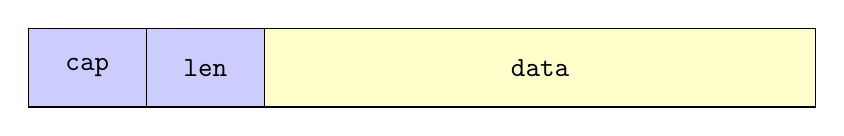
\begin{tikzpicture}[
    cell/.style={
        draw, 
        minimum height=1cm, 
        font=\ttfamily,
        inner sep=0pt,
        outer sep=0pt,
        node distance=0pt
    },
    bluecell/.style={cell, fill=myblue, minimum width=1.5cm},
    yellowcell/.style={cell, fill=myyellow, minimum width=7cm}
]

\node[bluecell] (cap) {cap};
\node[bluecell, right=of cap] (len) {len};
\node[yellowcell, right=of len] (data) {data};

\end{tikzpicture}
\end{document}
